\documentclass{scrartcl}
\usepackage[utf8]{inputenc}
\usepackage[english]{babel}
\usepackage{caption}
\usepackage{subcaption}
\usepackage{listings}
\usepackage{pdfpages}
\usepackage{amsmath,amssymb}
\usepackage{siunitx}
\usepackage{hyperref}
\usepackage{mhchem}
\usepackage[section]{placeins}
\usepackage[activate, protrusion=true, expansion=true]{microtype}
\usepackage[left=2.5cm, right=2.5cm, bottom=2.5cm, top=2.5cm]{geometry}
\usepackage{libertine}
\usepackage{longtable}

\renewcommand{\floatpagefraction}{.9}

\definecolor{mygreen}{rgb}{0,0.6,0}
\definecolor{mymauve}{rgb}{0.58,0,0.82}
\definecolor{mygray}{rgb}{0.5,0.5,0.5}
\lstset{backgroundcolor=\color{white},
  keepspaces=true,
  captionpos=b,
  keywordstyle=\color{blue},
  language=matlab,
  stringstyle=\color{mymauve},
  tabsize=2,
  numbers=left,                    % where to put the line-numbers; possible values are (none, left, right)
  numbersep=5pt,                   % how far the line-numbers are from the code
  numberstyle=\tiny\color{mygray},
  basicstyle=\footnotesize,        % the size of the fonts that are used for the code
  breakatwhitespace=false,         % sets if automatic breaks should only happen at whitespace
  breaklines=true,                 % sets automatic line breaking
  commentstyle=\color{mygreen},    % comment style
  deletekeywords={input},            % if you want to delete keywords from the given language
}

\newcommand*{\matlabcode}[3]{\begin{figure}[h!]\lstinputlisting[caption=#2, label=#3]{#1}\end{figure}}

\subtitle{System Identification (ME421)}
\title{Computer Exercises 1: Nonparametric Methods}
\author{\textsc{Julia Krottenthaler} \and \textsc{Arne Sachtler}}
\date{Fall 2018 - EPFL}

\begin{document}
\maketitle
\tableofcontents
\section{Step Response}

Figure~\ref{fig:testmodel} shows the modelled system, which will be used for the system identification exercises.
\textcolor{red}{TODO: is this a reasonable choice question}
Figure~\ref{fig:responses} shows the step and impulse response for the system. On the left hand side the noise is included, the right hand side shows the responses without noise.

\begin{figure}[h]
	\centering
	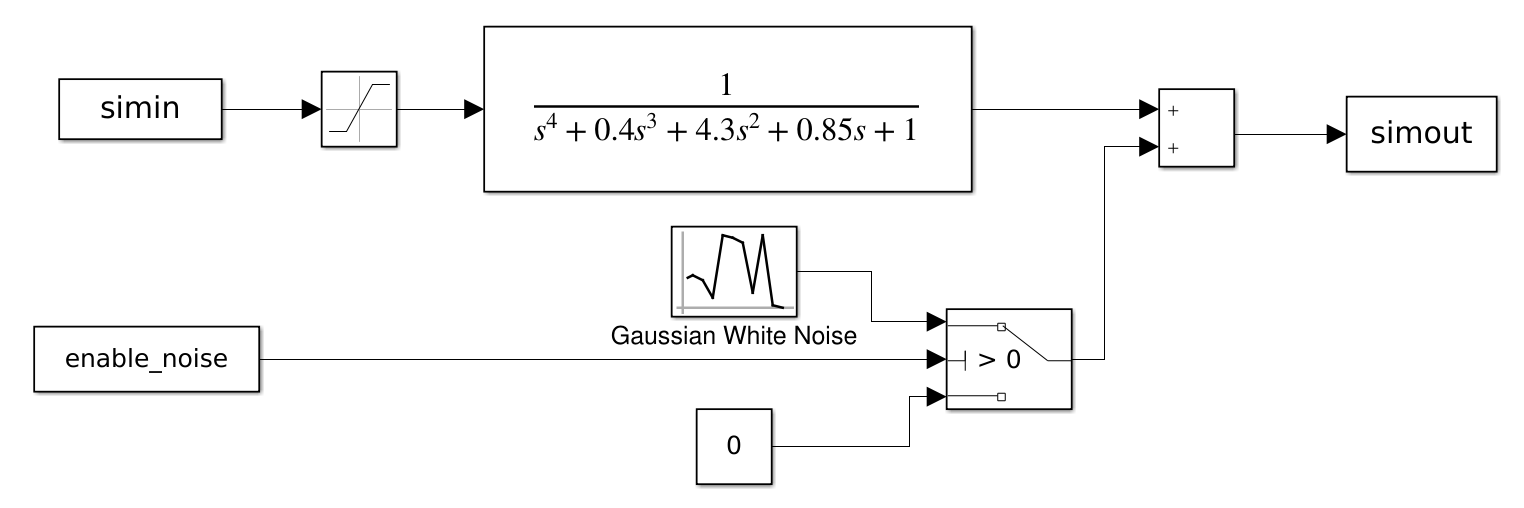
\includegraphics[height=4cm]{figures/systemmodel.png}
	\caption{Simulink model of the test system}\label{fig:testmodel}
\end{figure}
\begin{figure}[h]
	\centering
	\begin{subfigure}{0.49\textwidth}
		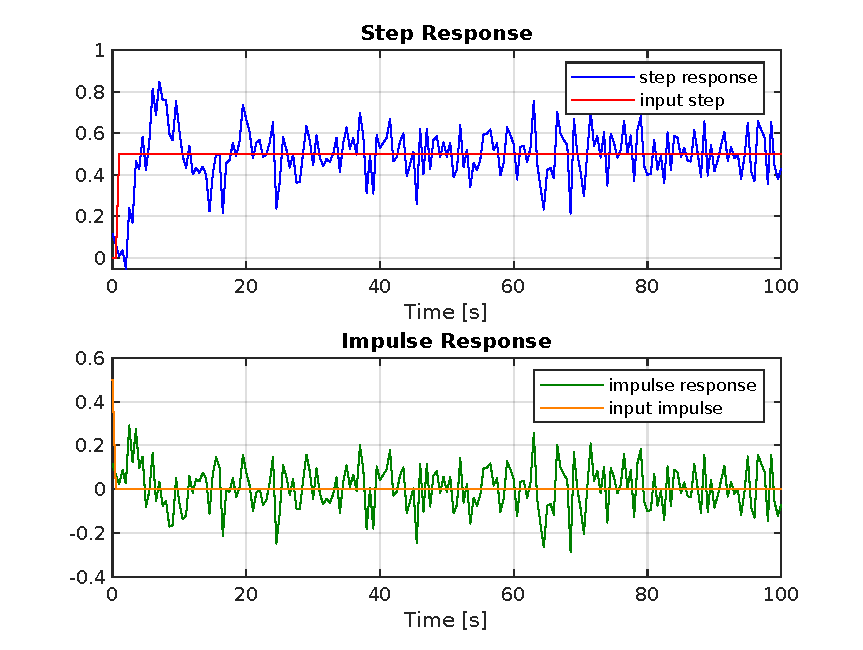
\includegraphics[width=\textwidth]{figures/noisy_responses.pdf}
		\subcaption{Noisy responses}
	\end{subfigure}
	\begin{subfigure}{0.49\textwidth}
		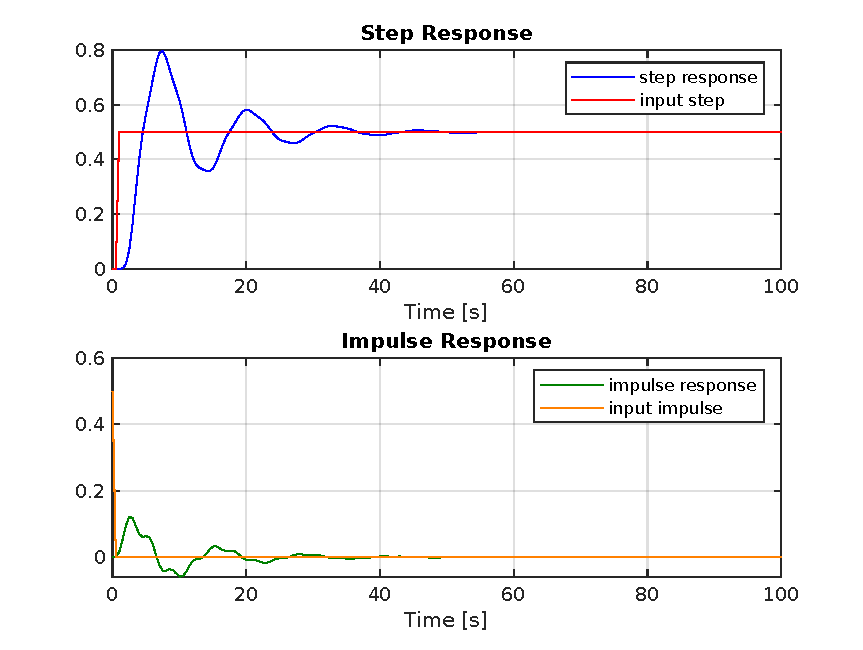
\includegraphics[width=\textwidth]{figures/noisefree.pdf}
		\subcaption{Responses without noise}
	\end{subfigure}
	\caption{Step and impulse responses of the test system with and without noise.}\label{fig:responses}
\end{figure}

\section{Auto Correlation of a PRBS signal}
In order to compute the cross-correlation of two discrete-time signals $u(k)$ and $y(k)$, we use 
\begin{equation}
	R_{uy}(h) = \frac{1}{M} \sum\limits_{k=0}^{M-1} u(k)y(k-h)\, .
\end{equation}
We assume two equal-length vectors for the signals $u$ and $y$. Let the length of the input signals be $N$, we choose the following interval for $h$
\begin{equation}
	h \in \{-H, \dots, -1, 0, 1, \dots, H\}\text{ , where } H = \left\lceil \frac{N}{2} \right\rceil \, .
\end{equation}
Using these definitions the cross-correlation can be computed in MATLAB using the code snippet shown in Listing~\ref{lst:corr}.

\matlabcode{../matlab/ce1/intcor.m}{Computing a discrete-time cross correlation of the signal u and y in matlab}{lst:corr}

In order to validate our implementation of the cross-correlation function, we used it to compute the autocorrelation two different test signals. 
Figure~\ref{fig:autocorr} shows the autocorrelation function of two different types of signals. 
On the left hand side (Figure~\ref{fig:autocorrPRBS}) there is a PRBS signal (length of the shift register is 4 and number of periods is 2) and its corresponding autocorrelation function. 
In addition, the figure on the right hand side (Figure~\ref{fig:autocorrSINUS}) displays a sinusoidal signal and its autocorrelation function.  

\begin{figure}[h]
	\centering
	\begin{subfigure}{0.49\textwidth}
		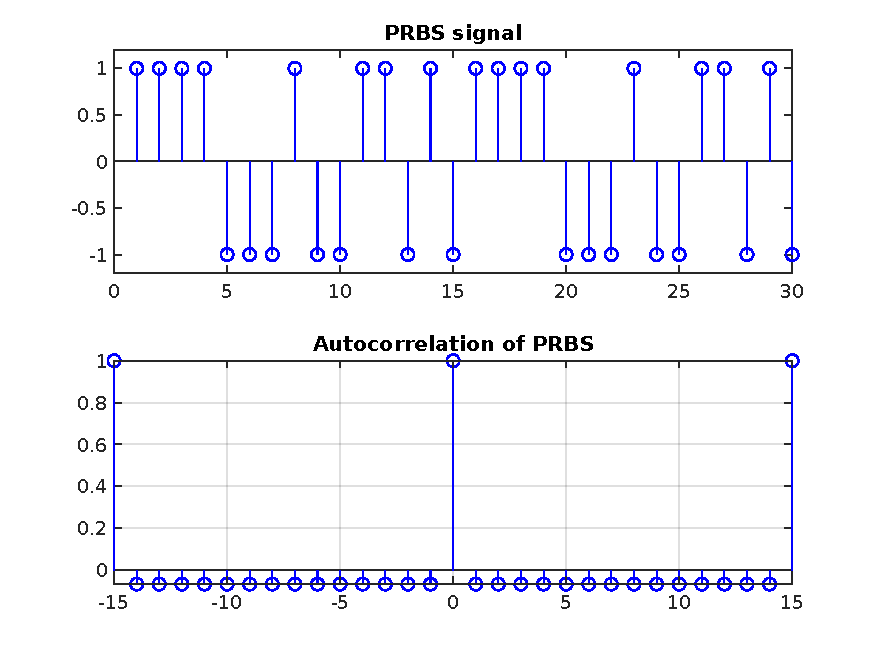
\includegraphics[width=\textwidth]{figures/prbs.pdf}
		\subcaption{PRBS signal}
		\label{fig:autocorrPRBS}
	\end{subfigure}
	\begin{subfigure}{0.49\textwidth}
		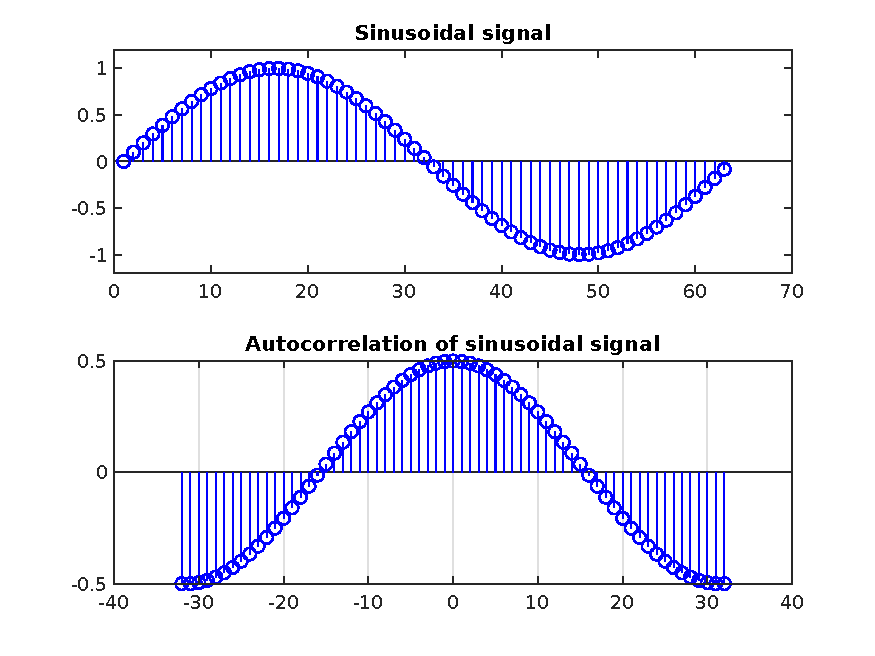
\includegraphics[width=\textwidth]{figures/sine.pdf}
		\subcaption{Sinus signal}
		\label{fig:autocorrSINUS}
	\end{subfigure}
	\caption{Two signals and their corresponding autocorrelation function}\label{fig:autocorr}
\end{figure}

\section{Impulse Response using the Deconvolution Method}\label{section:numdec}
In this exercise the deconvolution method is used in order to estimate the impulse response of a system.
We use digital random white noise signal, feed it to the model and record the system's response.
As an input signal we generate a random signal with the \verb|rand| command (Figure~\ref{fig:inout}).
In order to create the random signal we use \verb|rand| and squeeze the output to the $[-0.5, 0.5]$ interval.
Figure~\ref{fig:inout} shows the input and the response of the model.
In total, we generate $200s$ of white noise and run the simulation.

\begin{figure}[h]
	\centering
	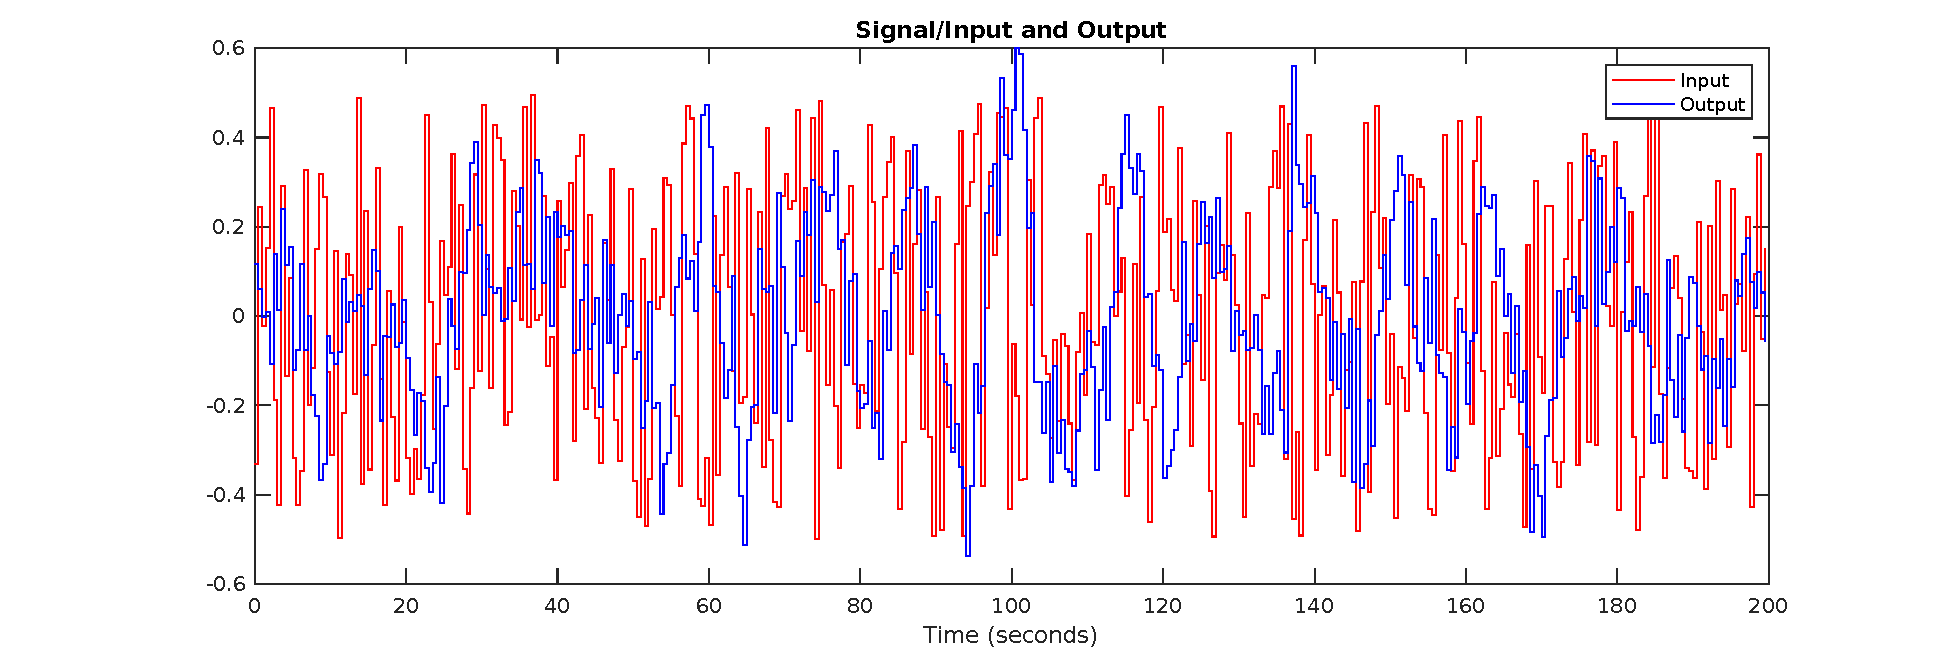
\includegraphics[height=5.5cm]{figures/input_output.pdf}
	\caption{Random input signal and output of the system}
	\label{fig:inout}
\end{figure}
Afterwards we can identify the discrete impulse response using the convolution relation
\begin{equation}
	y(k) = \sum\limits_{j=0}^{k} g(j)u(k-j) \text{ for } k=0,1,2,.. 
\end{equation}
or in a matrix form
\begin{equation}
	Y = U \Theta\, .
\end{equation}
Here, $U$ is an asymmetric (lower) triangular Toeplitz matrix.
Then, $\Theta$ can then be calculated using
\begin{equation}
	\Theta = U^{-1} Y.
\end{equation}
However, this approach does not lead to a good solution as the matrix $U$ is poorly conditioned and very close to singular.
Therefore, the inversion is highly numerically unstable and we don't get a proper result for the discrete impulse response as shown in Figure~\ref{fig:originalimpulse}.

In order to fix the numerical problem, we shorten the total length of the impulse response by assuming $g(k) = 0$ for $k \geq K$ and we obtain $Y = U_{K} \Theta_{K}$ by removing the last $N-K$ columns of $U$ and the last $N-K$ rows of $\Theta$. 
This equation can be solved in the least squares sense using the Moore-Penrose pseudo inverse $U_{K}^+$ of $U_{K}$
\begin{equation}
	\Theta_{K} = (U^{T}_{K} U_{K})^{-1} U^{T}_{K} Y = U_{K}^{+} Y.
\end{equation}
In MATLAB we can compute the least squares solution by simply using the backslash operator.
As the true impulse response is approximately zero after $75 s$, we decided to set $K = 150$. Thus, the obtained impulse response can be seen in Figure~\ref{fig:impulseresponse}. The result is similar to the true impulse response of the signal, which we compute using the \verb|impulse| command in MATLAB.
Note that we of course do not know the length of the impulse response for arbitrary systems to be identified. 
Here, other methods to determine the main time constants or systematic evaluation of different target lengths $K$ must be employed.
Listing~\ref{lst:numdec} shows our implementation in MATLAB.
\matlabcode{../matlab/ce1/estimate_impulse_response_numdec.m}{Estimator of the impulse response via numerical deconvolution in MATLAB.}{lst:numdec}
\begin{figure}[h]
	\centering
	\begin{subfigure}{.49\textwidth}
		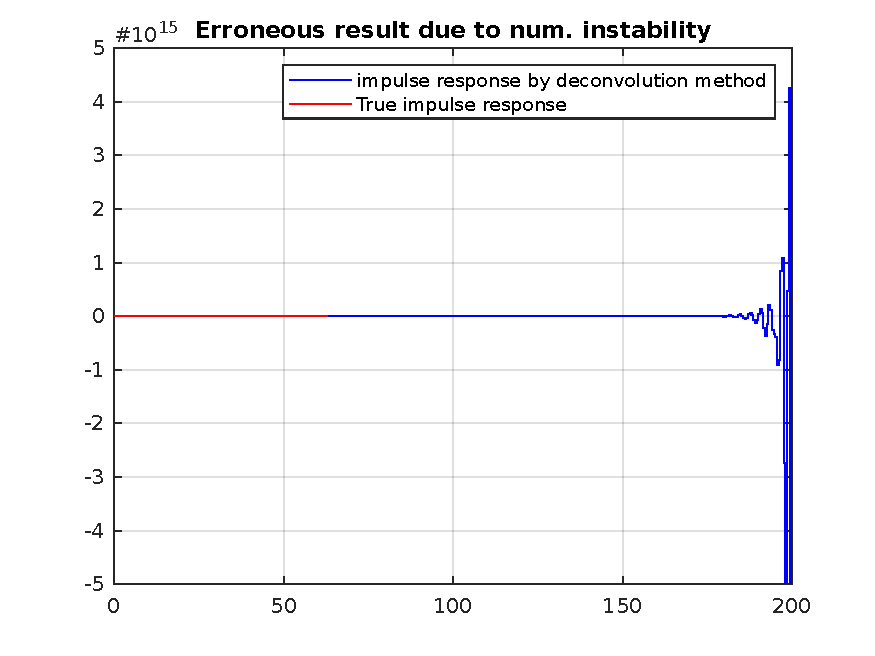
\includegraphics[width=\textwidth]{figures/original_impulse_response.pdf}
		\subcaption{Poor estimate of the impulse response due to the inversion of the poorly conditioned input matrix.}
		\label{fig:originalimpulse}
	\end{subfigure}
	\begin{subfigure}{.49\textwidth}
		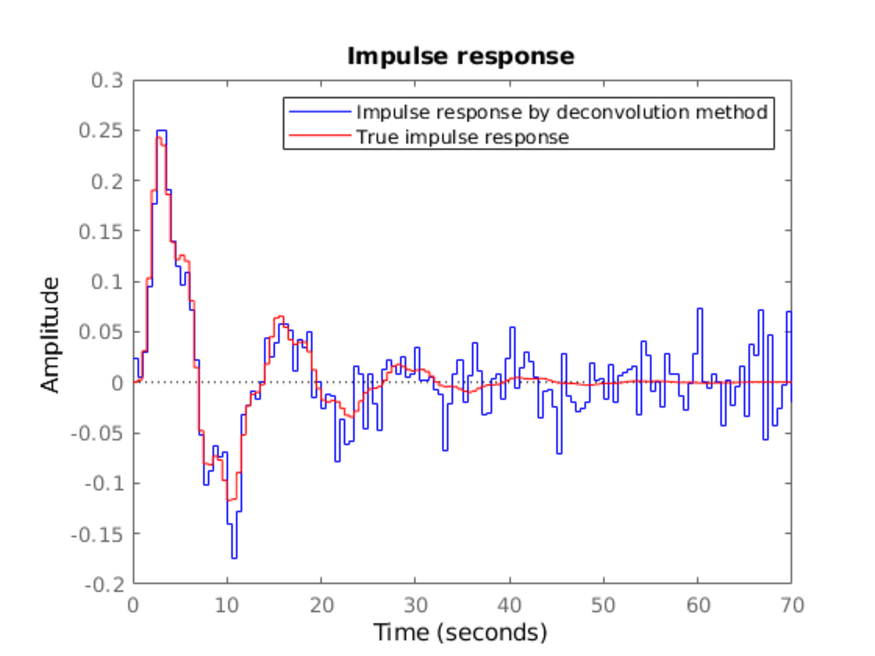
\includegraphics[width=\textwidth]{figures/impulse_response.pdf}
		\subcaption{Better estimate of the impulse response by constraining the length of the discrete finite impulse response.}
		\label{fig:impulseresponse}
	\end{subfigure}
	\caption{Impulse response by deconvolution method with random input signal}\label{fig:deconvolution}
\end{figure}
\noindent We get a 2-norm of the error vector as
\begin{equation}\label{eq:2-norm}
	E(\hat{g}) = \sqrt{\sum\limits_{k=0}^K \left(g(k) - \hat{g}(k)\right)^2}
\end{equation}
of $E(\hat{g}) = 0.22$.

\section{Impulse Response by Correlation Approach}
We generate a PRBS signal with $4$ periods in a $7$bit shift register model.
Afterwards, the PRBS signal is applied to the system.
First we compute the cross-correlation between the input and the output signal $R_{uy}(h)$ and the auto-correlation of the input signal $R_{uu}(h)$ using the previously implemented \texttt{intcor} function and MATLAB's \texttt{xcorr} function. The results are shown in Figure~\ref{fig:cross_correlations}.
\begin{figure}[h]
	\centering
	\begin{subfigure}{0.6\textwidth}
		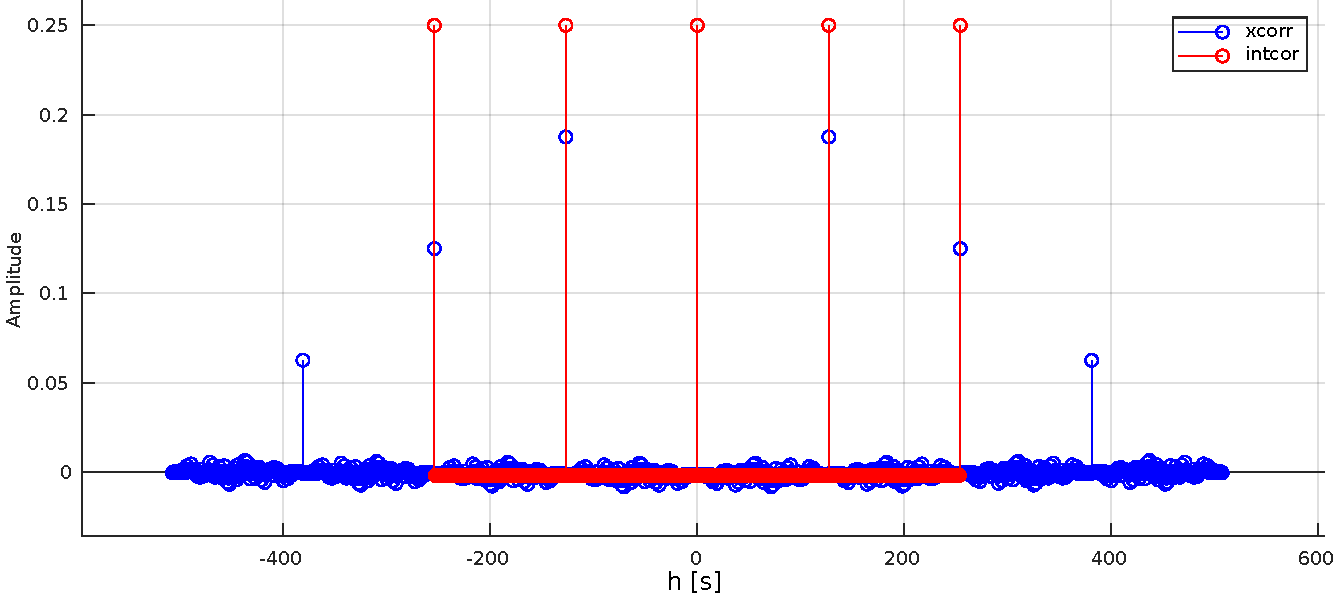
\includegraphics[width=\textwidth]{figures/ac.pdf}
		\subcaption{Auto-correlation $R_{uu}(h)$}
		\label{fig:cc_ac}
	\end{subfigure}
	\begin{subfigure}{0.6\textwidth}
		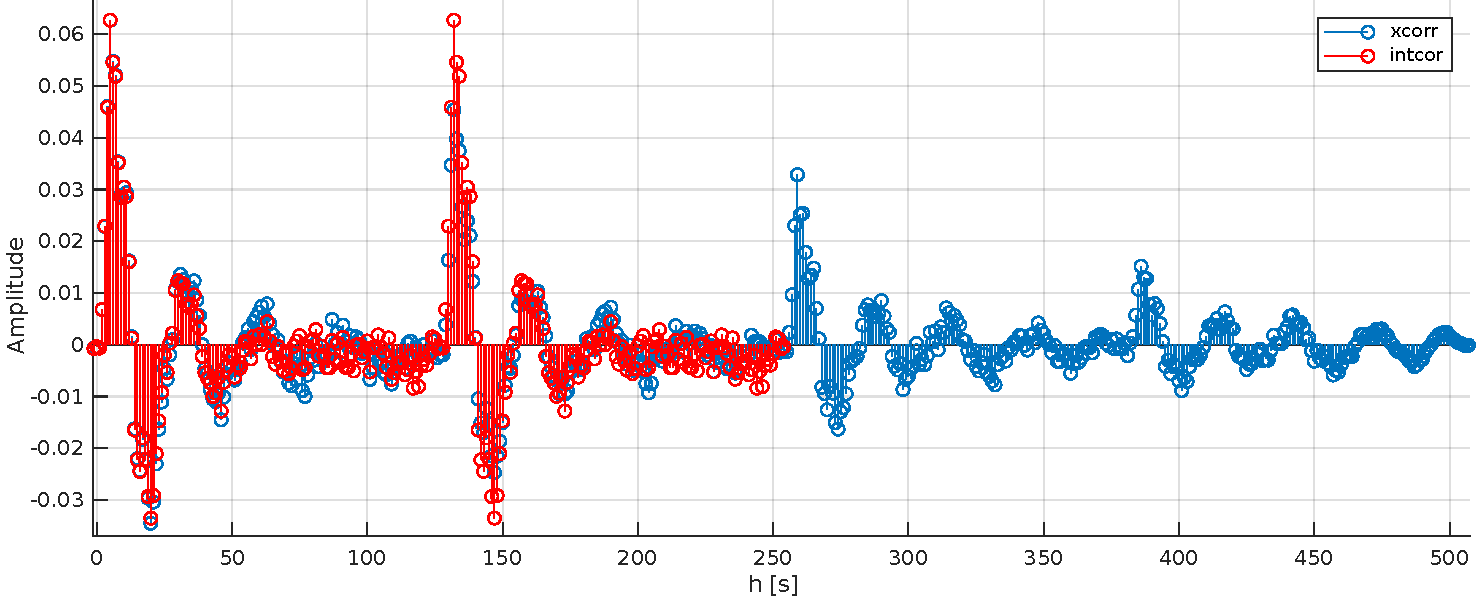
\includegraphics[width=\textwidth]{figures/cc.pdf}
		\subcaption{Cross-correlation $R_{yu}(h)$, (zoomed and truncated)}
		\label{fig:cc_cc}
	\end{subfigure}
	\caption{Correlation signals computed from input and output signal.}\label{fig:cross_correlations}
\end{figure}

The function \texttt{intcor} and \texttt{xcorr} yield the same results at $0$, but different results for the remaining values on the time-axis.
Generally, if $N$ is the signal length, \texttt{intcor} provides a correlation signal with a length of $N+1$ for $N$ even and $N+3$ for $N$ odd.
MATLAB's implementation yields a significantly longer signal and the correlation sum is weighted by some function of $h$.
Because of that, for $h\neq0$ MATLAB's \texttt{xcorr} shows a non-constant value for the PRBS auto-correlation while \texttt{intcor} does.
Figure~\ref{fig:correlation_impulse_responses} shows the resulting impulse responses in comparison to the ground truth.
We additionally compared the result of the simplified algorithms for white input signals.
As PRBS is not exactly white, we get lower performance for the simplified version and we have to apply numerical deconvolution to improve.
We implemented the different approaches in the same function, an optional parameter allows to choose one of the methods. 
Our implementation is presented in Listing~\ref{lst:corr_approach}.
\begin{figure}[h!]
	\centering
	\begin{subfigure}{0.49\textwidth}
		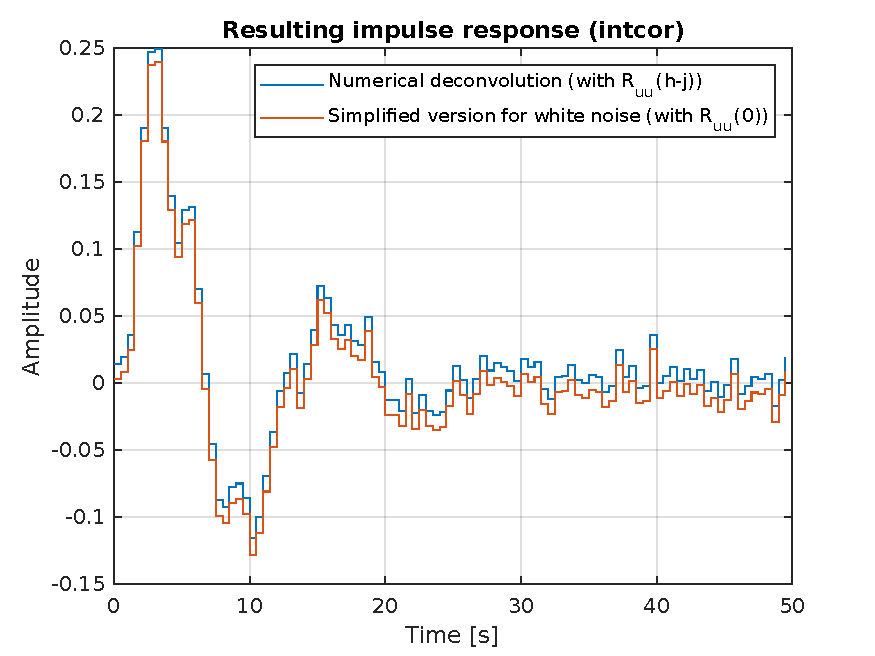
\includegraphics[width=\textwidth]{figures/impulse_response_intcor.pdf}
		\subcaption{Resulting impulse response using intcor.}
		\label{fig:impulse_response_intcor}
	\end{subfigure}
	\begin{subfigure}{0.49\textwidth}
		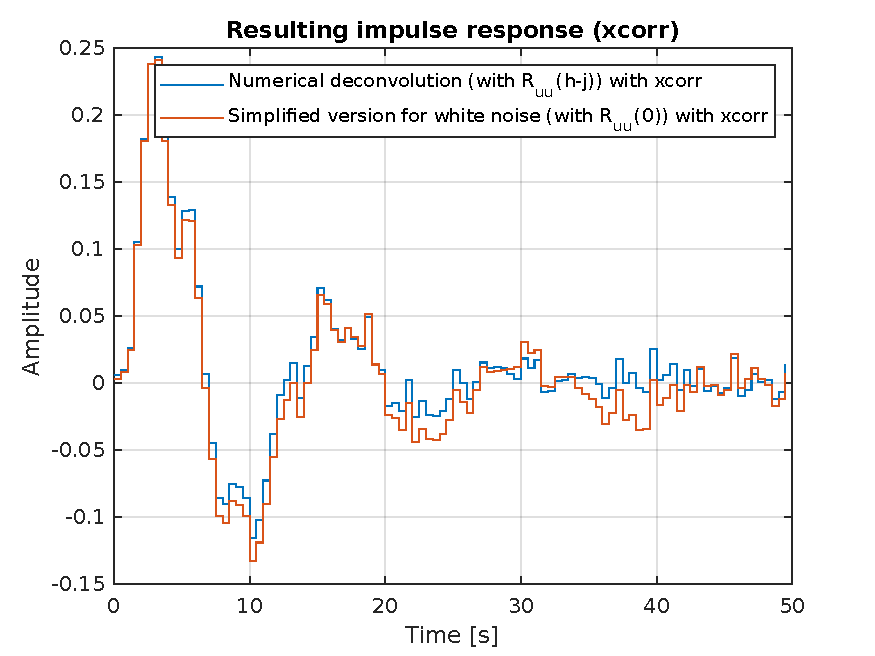
\includegraphics[width=\textwidth]{figures/impulse_response_xcorr.pdf}
		\subcaption{Resulting impulse response using xcorr.}
		\label{fig:impulse_response_xcorr}
	\end{subfigure}
	\begin{subfigure}{\textwidth}
		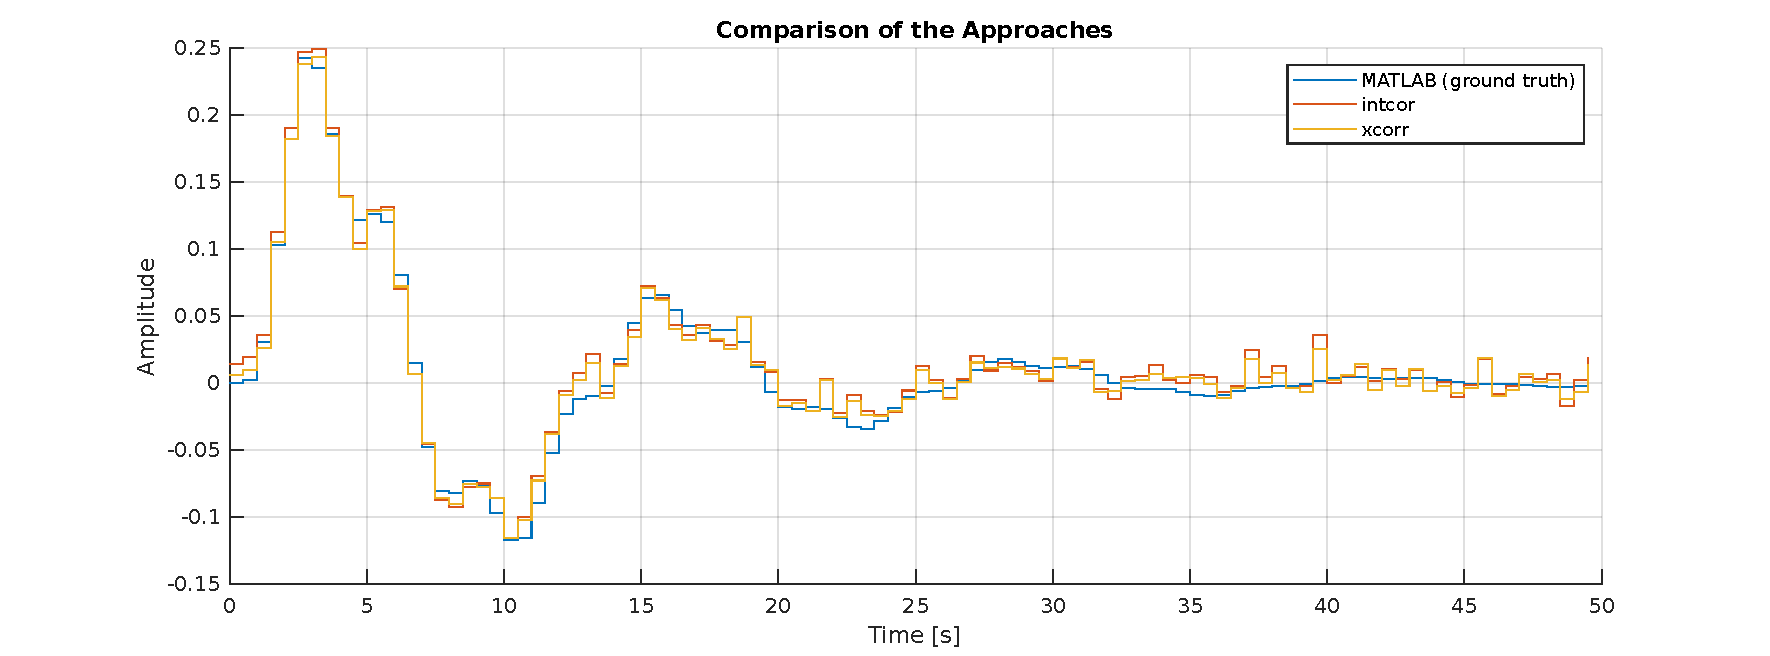
\includegraphics[width=\textwidth]{figures/impulse_response_comparison.pdf}
		\subcaption{Comparison with ground truth impulse reponse.}
		\label{fig:impulse_response_comparison}
	\end{subfigure}
	\caption{Comparison of the identified impulse response with the ground truth.}\label{fig:correlation_impulse_responses}
\end{figure}

\pagebreak
Table~\ref{tab:correlation_appraoch_errors} shows the 2-norm of the errors between ground truth impulse response and the estimated results.
The 2-norms of the errors are computed based on \eqref{eq:2-norm}.
We additionally compare the result to the estimate of the numerical deconvolution algorithm developed in the previous section.
Note that, in contrast to the previous section, we now apply a PRBS signal instead of random white noise to the system.
We observe that the error of the numerical deconvolution approach is significantly smaller (approx. half as large) than in the previous section. 
As we use the same impulse reponse length $K$, the smaller error is due to the better eligible PRBS signal.
The comparison shows that the correlation approach with the \texttt{xcorr} correlation function shows the lowest error, while the correlation approach with the \texttt{intcor} function performs worst.
The performance of the previous numerical deconvolution of the input and output signals directly is between the new approaches of this section.
\begin{table}[h]
	\centering
	\begin{tabular}{l|c}
	\hline
	\hline
	\textbf{Approach} & \textbf{2-norm of error}\\
	\hline
		correlation approach using \texttt{intcor} & $0.13$ \\
		correlation approach using \texttt{xcorr} & $0.10$ \\\hline
		numerical deconvolution (1.\ref{section:numdec}) & $0.12$\\
	\hline
	\hline
	\end{tabular}
	\caption{Errors of the estimates of the impulse responses compared to the ground truth impulse response obtained by the MATLAB command. We compare the correlation approach algorithm for the correlation functions \texttt{intcor} and \texttt{xcorr} as well as the numerical deconvolution approach from the previous section.}
	\label{tab:correlation_appraoch_errors}
\end{table}

\matlabcode{../matlab/ce1/estimate_impulse_response_corr.m}
{Estimator of the impulse response via the correlation approach.}
{lst:corr_approach}
\section{Frequency Domain Identification using a Periodic Signal}
In this task we want to use the Fourier analysis method to identify the frequency response of our model shown in Figure~\ref{fig:testmodel}. 
For the frequency domain identification we use $8$ periods of a PRBS signal generated by a $8$-bit shift-register.
Consequently, our total signal length is $N=2040$. The sampling frequency is at $\SI{2}{\hertz}$.
In order to get a good trade off between the resolution of the estimates (samples per period $M = 2^n -1$) and the impact of measurement errors (number of periods $p$) we decide to choose a signal with 8 periods $p=8$ in a 8 bit $n=8$ shift register.

First we compute the Fourier transform of the input and the obtained output signal of our system using the \texttt{fft} command in MATLAB for each period. To reduce the measurement error we average the Fourier series coefficients but we ignore the first period
\begin{align}\label{eq:fft_average}
	 Y(n) = \frac{1}{p}\sum\limits_{i=2}^p Y_i (n) \quad \quad n = 1,2,\ldots,M
 \intertext{and} 
	U(n) = \frac{1}{p}\sum\limits_{i=2}^p U_i (n) \quad \quad n = 1,2,\ldots,M .
\end{align}
In addition we calculate the frequency response $ G(e^{j \omega_n}) = Y(n)/ U(n)$. 
The results can be seen in Figure ~\ref{fig:ffts_diff}.
In order to determine the effect of noise to the frequency response, we compared the spectra of the system response to a PRBS signal and to a constant-zero input.
We can observe, that for frequencies higher than $\approx 2.5\frac{rad}{s}$ the signal is hidden in the noise and consequently we expect in poorer identification result in the frequency range higher than $\omega = 2.5\frac{rad}{s}$.

\begin{figure}[h!]
	\centering
	\begin{subfigure}{0.49\textwidth}
		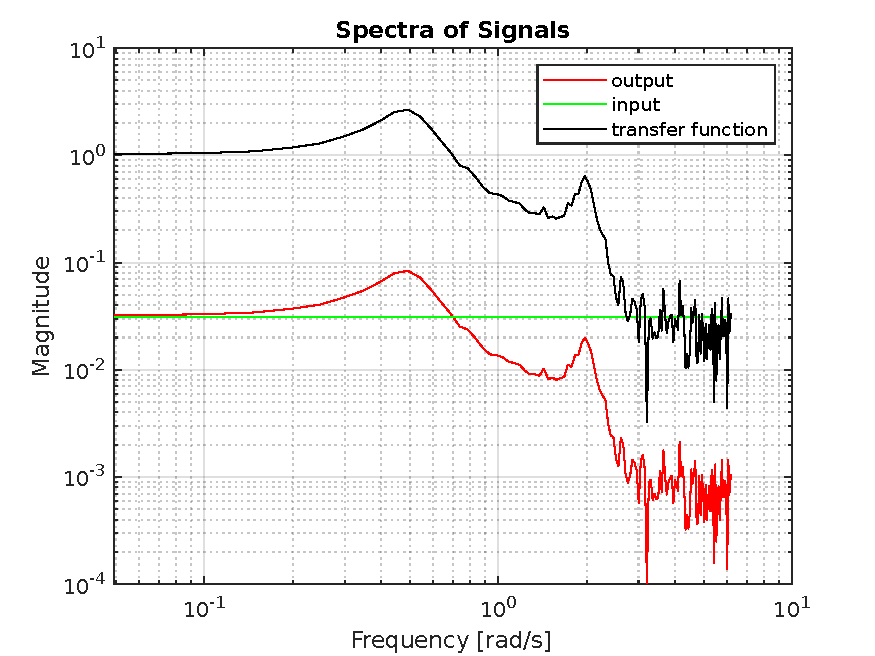
\includegraphics[width=\textwidth]{figures/ffts.pdf}
		\subcaption{input signal $U$, the output signal $Y$ and the transfer function $G$}\label{fig:ffts_diff}
	\end{subfigure}
	\begin{subfigure}{0.49\textwidth}
		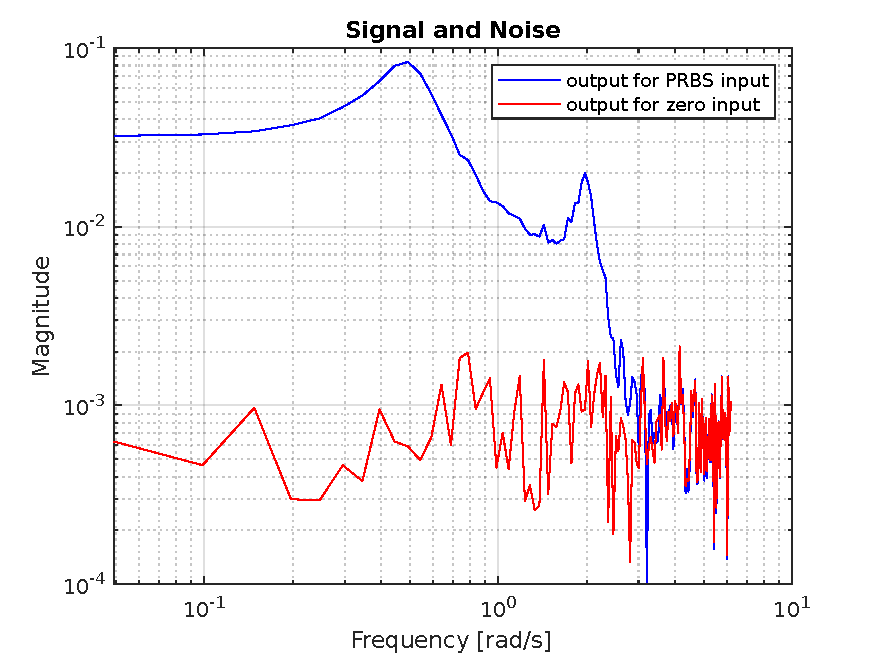
\includegraphics[width=\textwidth]{figures/ffts_snr.pdf}
		\subcaption{output signal for PRBS input and zero input}\label{fig:ffts_snr}
	\end{subfigure}
	\caption{Spectra of different signals. On the left we show the spectra of the input and output signals as well as the transfer function when applying the PRBS signal to the system. On the right we apply to different signals, a PRBS signal and a constant-zero signal, to the system and show the spectra of the system response. We can observe, that for high frequencies the system frequency response hides in the noise.}
\end{figure}
Afterwards we compute the frequency vector for one period
\begin{equation}\label{eq:f_vector}
	\left[ 0, \frac{\omega_s}{M},\frac{2\omega_s}{M}, \ldots, \frac{(M-1)\omega_s}{M} \right] .
\end{equation}
This vector is then used to generate a frequency-domain model using the MATLAB \texttt{frd} command. 
Finally, we compare the obtained Bode diagram of the identified model with the true one. Figure ~\ref{fig:resp_noiseless} shows the frequency response without noise. 
As we use a periodic signal, the truncation error is suppressed and the identified model approaches the true one (neglecting numerical errors) exactly. 
Figure ~\ref{fig:resp_noise} shows the frequency response applying a PRBS signal with the noise block switched on.
As we predicted based on the spectra of the output signals in Figure~\ref{fig:ffts_snr}, the estimated frequency response becomes poor for frequencies higher than $\approx 2.5 \frac{rad}{s}$.
\begin{figure}[h]
	\begin{subfigure}{0.45\textwidth}
		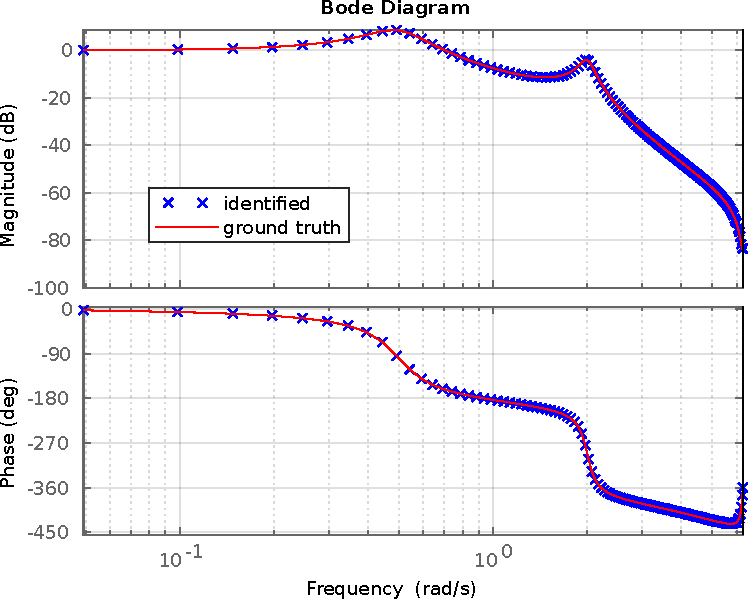
\includegraphics[width=\textwidth]{figures/resp_nonoise.pdf}
		\subcaption{Identified frequency response and true response with noise block switched off.}
		\label{fig:resp_noiseless}
	\end{subfigure}
	\hspace*{0.05\textwidth}
	\begin{subfigure}{0.45\textwidth}
		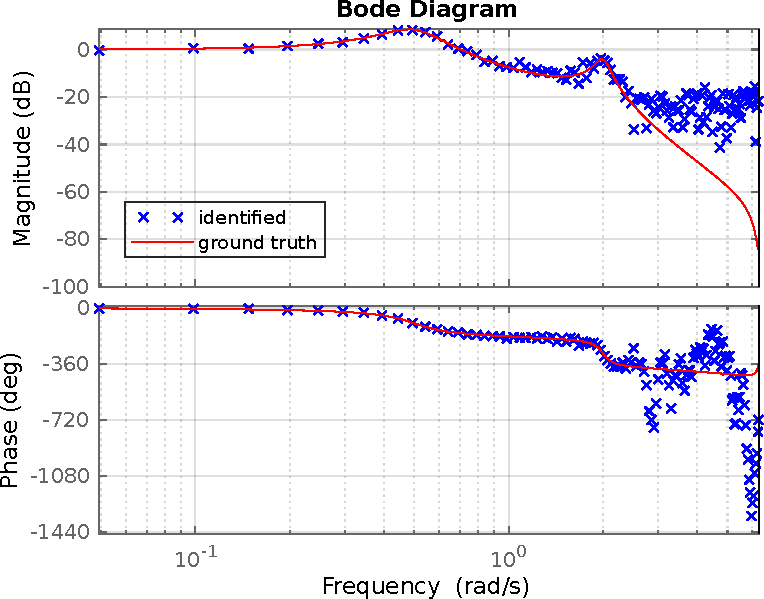
\includegraphics[width=\textwidth]{figures/resp_noise.pdf}
		\subcaption{Identified frequency response and true response with noise block switched on.}
		\label{fig:resp_noise}
	\end{subfigure}
	\caption{Comparison of the frequency response of identified model with the true one}\label{fig:f_resp}
\end{figure}
\matlabcode{../matlab/ce1/estimate_frequency_response.m}
{{Compute frequency response of the system to be identified using an average of Fourier transforms of each period. The first period is skipped as we wait for transience to vanish. Additionally, the frequency vector is computed.}}
{lst:freq_resp}

\section{Frequency Domain Identification using a Random Signal}

\end{document}
